\documentclass[11pt]{article}
\usepackage{float}

\usepackage{acl}
\usepackage{times}
\usepackage{latexsym}
\usepackage{microtype}
\usepackage{booktabs}
\usepackage{graphicx}
\usepackage{multirow}
\usepackage{amsmath}
\usepackage{amssymb}
\usepackage{xcolor}
\usepackage{hyperref}
\usepackage{appendix}
\usepackage{enumitem}
\usepackage{tcolorbox}
\usepackage{xcolor}
\tcbuselibrary{breakable,skins}

\definecolor{simple}{HTML}{F0C040}
\definecolor{standard}{HTML}{50C878}
\definecolor{detailed}{HTML}{4A90E2}

\newtcolorbox{prompttextbox}[2]{
  colback=white,           % 正文：纯白底色
  colframe=#2,             % �� 边框和标题背景：读取第二个大括号的颜色
  coltitle=white,          % 标题：纯白文字
  fonttitle=\bfseries\small,
  title={#1},              % �� 标题文字：读取第一个大括号的文字
  breakable,
  boxrule=0.4pt,
  left=6pt, right=6pt, top=4pt, bottom=4pt,
  toptitle=4pt, bottomtitle=4pt,
}

% CJK support for Chinese examples
\usepackage{xeCJK}
\setCJKmainfont{Noto Serif CJK SC}[BoldFont=Noto Serif CJK SC Bold]
\setCJKsansfont{Noto Sans CJK SC}
\setCJKmonofont{Noto Sans Mono CJK SC}

% EMNLP 2026 formatting
\newcommand\BibTeX{Bib\TeX}

\title{RewritingBench: A Diagnostic Benchmark for Chinese Text Rewriting Evaluation}

\author{
  Anonymous EMNLP Submission
}

\date{}

\begin{document}

\maketitle

\begin{abstract}
Evaluating text rewriting quality remains challenging, especially in Chinese, where no validated benchmark exists and automatic metrics are unreliable. We present RewritingBench, the first human-annotated benchmark for Chinese rewriting, containing 730 pairs rated by three annotators (inter-annotator Spearman $\rho \approx 0.86$). Our analysis reveals a striking pattern: common metrics—including BLEU, ROUGE, and SBERT—negatively correlate with human judgments ($\rho$ from $-$0.28 to $-$0.60), due to a misalignment between similarity-based metrics and human notions of quality. As an alternative, pairwise preference learning bridges this gap: a LoRA fine-tuned 8B model achieves $\rho=0.688$, outperforming pointwise scoring ($\rho=0.645$), zero-shot models up to 235B parameters ($\rho \leq 0.406$), and all general-purpose evaluators. We further validate this approach through downstream data filtering, showing that evaluator-guided selection can improve mean rewrite quality by 47\%.  Our benchmark and evaluation methodology provide a foundation for advancing Chinese rewriting assessment.
\end{abstract}

% ============================================================
\section{Introduction}
\label{sec:intro}
% ============================================================


Text rewriting transforms a source text into a semantically equivalent but stylistically different output, including paraphrasing, style transfer, simplification, and formality adaptation. While large language models (LLMs) have improved fluent rewriting, evaluating \emph{quality} remains challenging~\citep{zheng2023judging, liu2024geval}.

Standard metrics such as BLEU~\citep{papineni2002bleu} and ROUGE~\citep{lin2004rouge} rely on surface overlap with references. However, rewriting is inherently divergent, as high-quality outputs typically require significant lexical and structural transformations while preserving core meaning. Consequently, overlap-based metrics often exhibit a misalignment with human judgment.
Recent LLM-based evaluators, such as G-Eval~\citep{liu2024geval} and Prometheus~2~\citep{kim2024prometheus2}, leverage semantic understanding for general-purpose assessment. Despite their promise, these models often lack the specialized alignment required for nuanced rewriting tasks, and their efficacy in the Chinese linguistic context remains largely unexplored.

In this work, we systematically investigate Chinese rewriting evaluation and find a striking result: all traditional metrics exhibit a negative correlation with human judgment (Spearman $\rho$ from $-0.28$ to $-0.60$). This reveals a fundamental misalignment where overlap-based metrics reward surface similarity over genuine quality.

\begin{figure}[t]
\centering
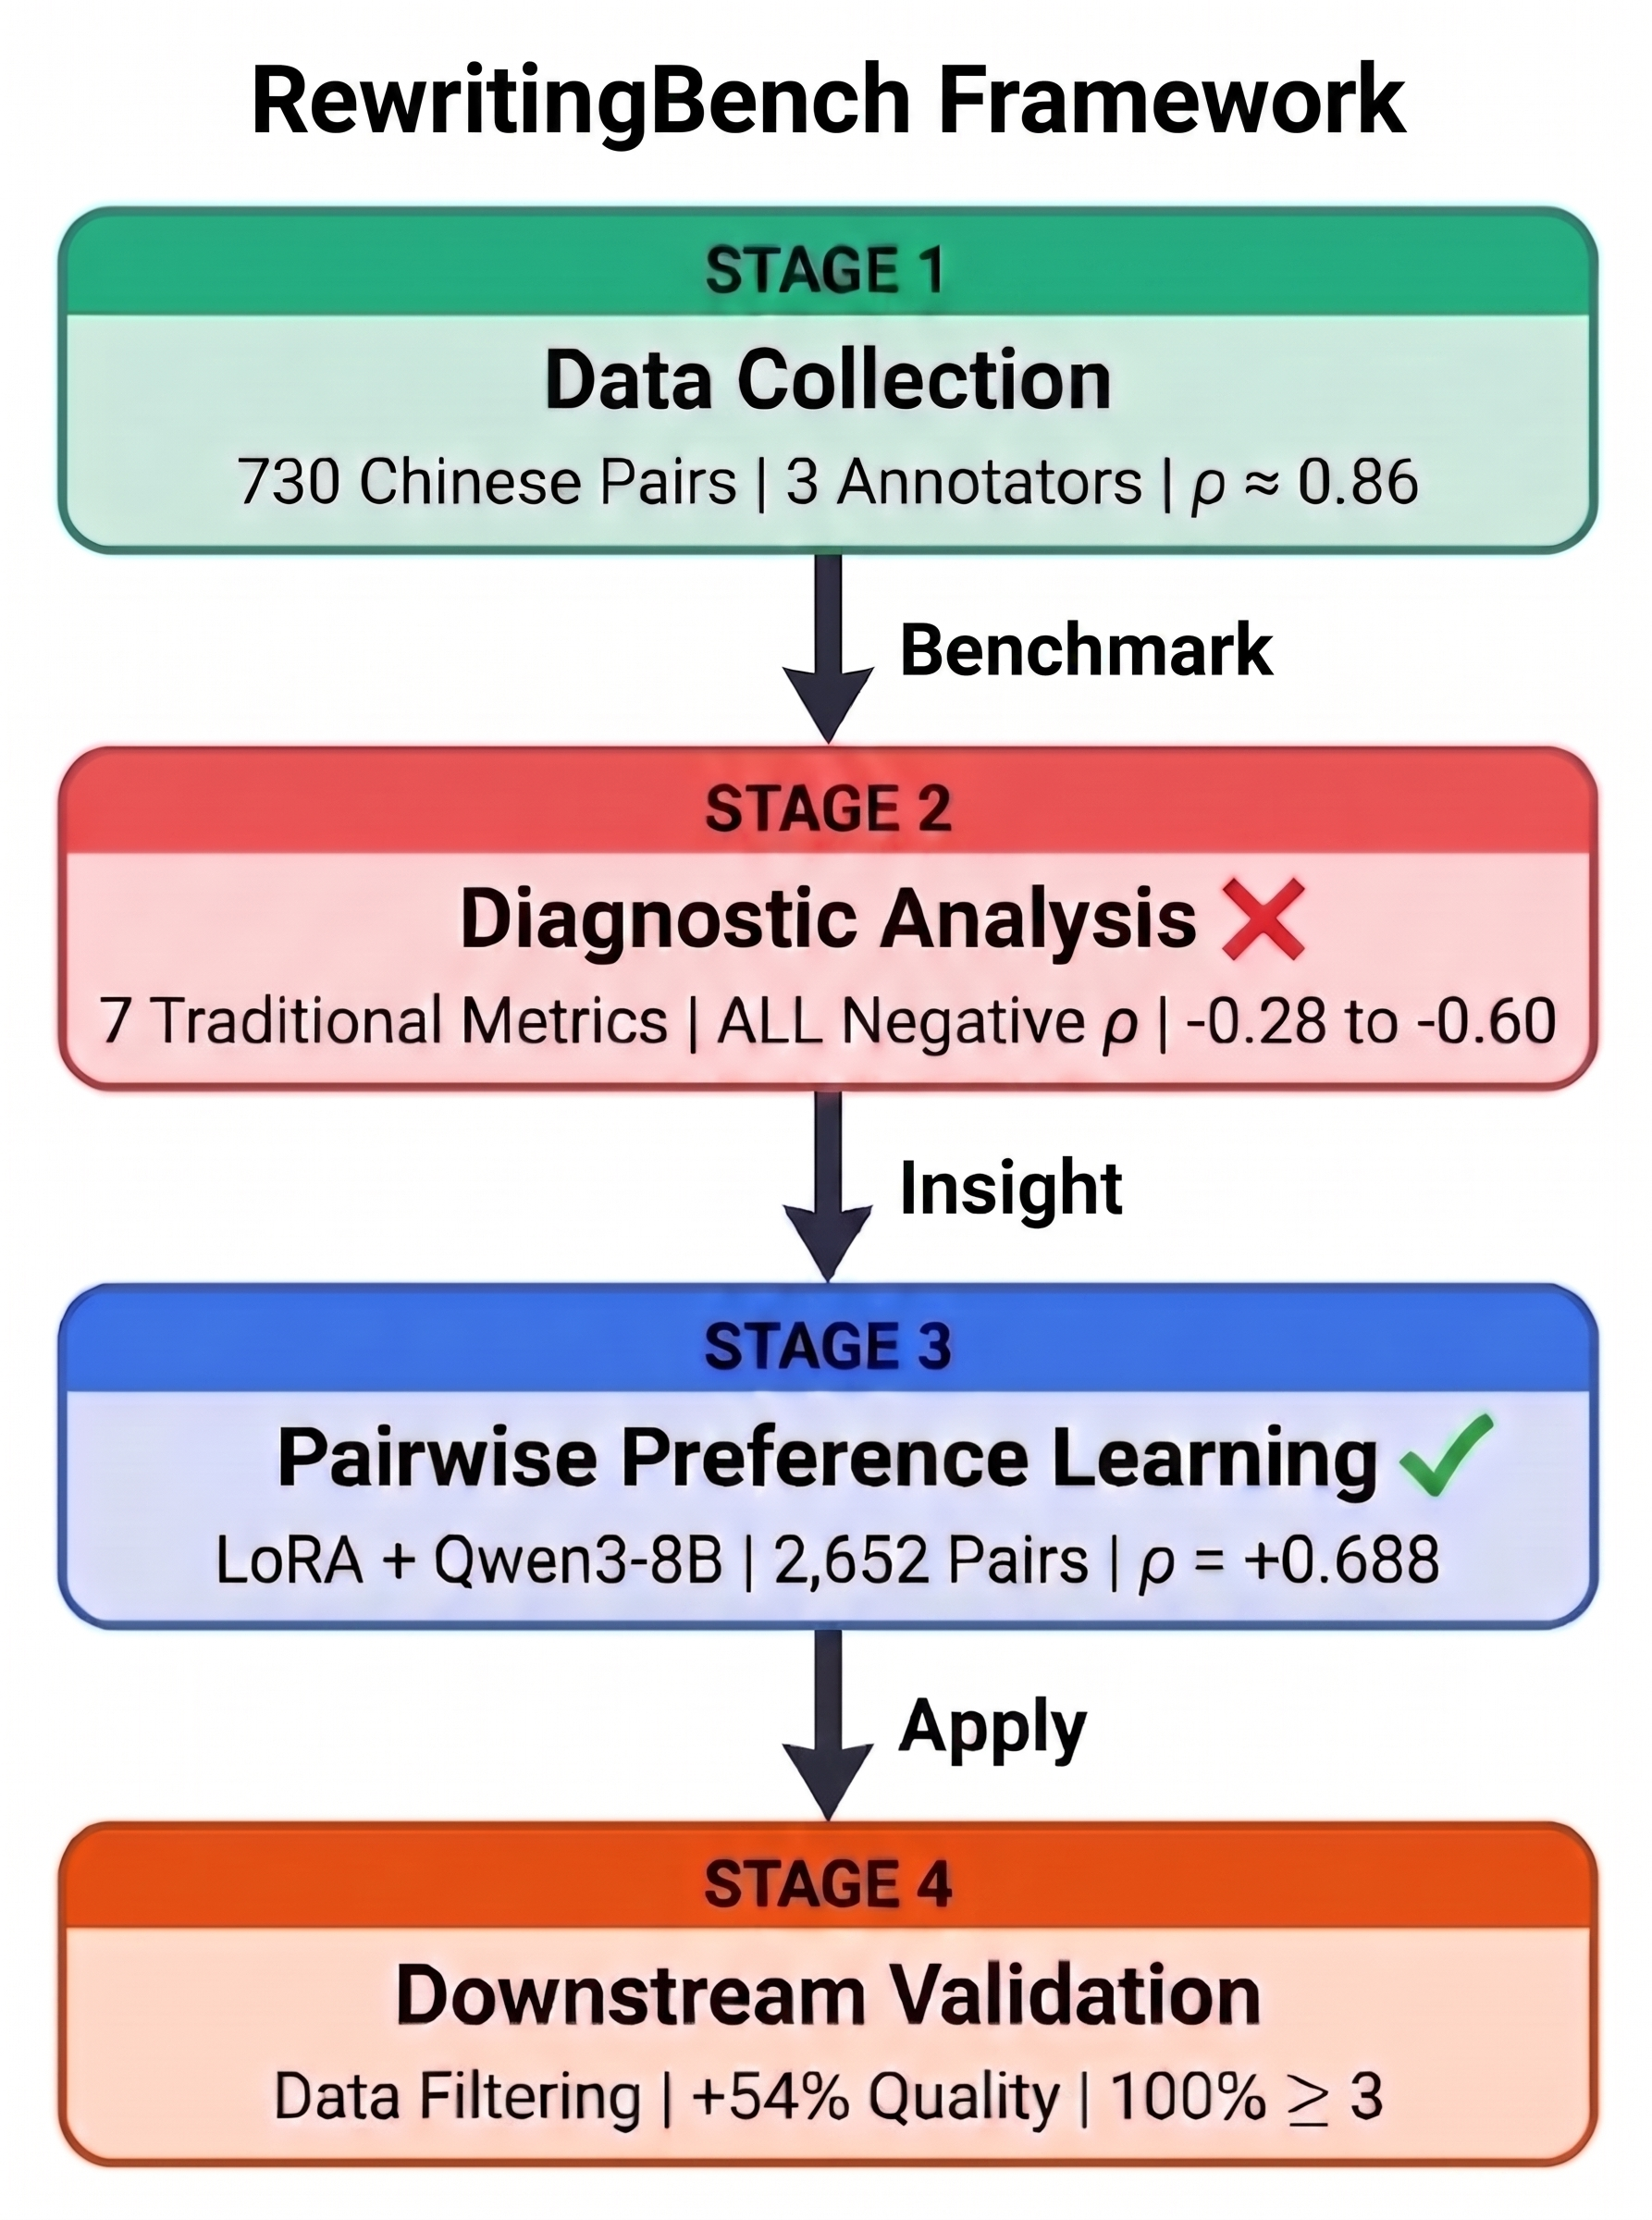
\includegraphics[width=0.85\columnwidth, height=6cm, keepaspectratio]{figures/ai_generated/framework_overview_v1.png}
\caption{Overview of the RewritingBench framework. From data collection (730 Chinese rewrite pairs) to diagnostic analysis, pairwise preference learning ($\rho$=0.688), and downstream validation.}
\label{fig:framework}
\end{figure}

To address this, we present RewritingBench (Figure~\ref{fig:framework}), the first human-annotated benchmark for Chinese rewriting quality. Our contributions are fourfold. First, we provide 730 annotated pairs (0--5 scale) with high agreement ($\rho \approx 0.86$). Second, we show that seven traditional text-overlap metrics systematically fail to capture quality ($p < 0.001$). Third, our pairwise preference learning approach (LoRA-tuned 8B) achieves $\rho=0.688$, substantially outperforming absolute scoring ($\rho=0.645$), zero-shot models up to 235B ($\rho \leq 0.406$), and Prometheus~2 ($\rho=0.124$). Fourth, evaluator-guided filtering improves mean rewrite quality by 47\% over random selection, demonstrating its real-world utility.

% Figure~\ref{fig:framework} provides an overview of the RewritingBench framework, from data collection through diagnostic analysis to pairwise preference learning and downstream validation.



% ============================================================
\section{Related Work}
\label{sec:related}
% ============================================================

\subsection{Text Rewriting Evaluation}

Traditional rewriting evaluation relies on overlap metrics like BLEU~\citep{papineni2002bleu} and ROUGE~\citep{lin2004rouge}, which are misaligned with rewriting since high-quality rewrites should \emph{differ} from the source rather than merely reproduce it. Embedding-based metrics such as SBERT~\citep{reimers2019sbert} improve semantic alignment, and methods like ParaScore~\citep{lan2023parascore} and \citet{alam2024generalized} consider paraphrase quality and multiple dimensions. \citet{jourdan-etal-2025-identifying} emphasize aligning metrics with human judgments in scientific text revision, but these approaches remain largely untested for Chinese rewriting.

\subsection{LLM-as-a-Judge}

The LLM-as-a-Judge paradigm offers a flexible alternative to reference metrics. G-Eval~\citep{liu2024geval} uses chain-of-thought prompting to produce structured evaluations, Prometheus~2~\citep{kim2024prometheus2} fine-tunes a 7B model for absolute and pairwise scoring, and Chatbot Arena~\citep{chiang2024chatbot} leverages human pairwise comparisons. However, in specialized domains like Chinese rewriting, these general-purpose evaluators often struggle, exhibiting biases~\citep{wang2024vlm} and rating inconsistencies~\citep{lee2025reliable} that require calibration.

\subsection{Pairwise Preference Evaluation}

Pairwise comparison has been studied as a more robust evaluation paradigm than absolute scoring, with \citet{kim2024prometheus2} finding higher agreement with human judgments in general NLP tasks. \citet{zheng2023judging} use it for LLM assessment, and recent work on generative selection~\citep{wang2024genrm} demonstrates that comparative scoring outperforms absolute scoring for best-of-N selection. However, its effectiveness for \emph{domain-specific} tasks such as Chinese text rewriting has not been systematically studied. Our work fills this gap by demonstrating a 6.26\% improvement from pairwise over absolute scoring on RewritingBench.

\subsection{Low-Resource Fine-Tuning}

Parameter-efficient fine-tuning methods enable adapting large models to specific tasks with limited computational resources.
LoRA~\citep{hu2022lora} injects trainable low-rank matrices into transformer layers, dramatically reducing the number of trainable parameters.
QLoRA~\citep{dettmers2024qlora} extends this with 4-bit quantization, enabling fine-tuning of large models on consumer GPUs.
These methods have proven effective for domain-specific adaptation~\citep{sun2024survey}, and we leverage them to create our rewriting evaluator with minimal computational cost.

% ============================================================
\section{Method}
\label{sec:method}
% ============================================================

\textbf{Task definition.}We study the evaluation of Chinese text rewriting quality: given a source text $s$ and a candidate rewrite $r$, the goal is to assign a score reflecting how well $r$ improves $s$ while preserving meaning. Our benchmark focuses on \emph{general-purpose text improvement rewrites} that enhance fluency, clarity, or readability without targeting a specific style. This reflects common real-world scenarios across genres (news, social media, literature, technical writing), assessing the overall quality of a rewrite. Formally, we define the evaluation function as:
\begin{equation}
    f: \mathcal{S} \times \mathcal{R} \rightarrow [0, 5]
\end{equation}

\subsection{Evaluation Framework}
\label{sec:eval_framework}

We define text rewriting quality along four complementary dimensions, scored on a 0–5 scale: \textbf{Semantic consistency} (preserve meaning without errors), \textbf{Syntactic reconstruction}  (structural changes beyond word substitution), \textbf{Lexical variation} (diverse yet natural vocabulary), and \textbf{Stylistic fidelity} (adherence to any target style). The final score is a holistic judgment integrating all dimensions. In our protocol, annotators provide only this unified rating, using the four dimensions as internal guidelines rather than separate scores.

\subsection{Training Data}

We collected 730 Chinese rewrite pairs, each consisting of a source text and a generated rewrite from various language models. Three trained annotators independently scored each pair on the 0–5 holistic quality scale, with high inter-annotator agreement (pairwise Spearman $\rho \approx 0.86$); We use the average of these ratings as the gold standard.  The dataset is split into 600 training pairs and 130 evaluation pairs (129 after removing one parsing issue) using stratified sampling by score to ensure balanced representation. The evaluation set closely reflects the full score distribution: 0 (15.5\%), 1 (27.9\%), 2 (24.8\%), 3 (20.2\%), 4 (9.3\%), 5 (2.3\%).

\subsection{Class-Balanced Training Strategy}
\label{sec:balanced}

A key challenge is the highly imbalanced score distribution (Score~0: 15\%, Score~5: 3\%), which causes mode collapse: training RewriteJudge on the original data leads to 82\% of predictions being Score~1 and near-zero correlation with human judgments ($\rho=0.253$). To mitigate this, we employ class-balanced oversampling to create a training set of 1,008 samples (168 per class) via random duplication and slight augmentation. This balancing is critical, transforming the model from making uniform predictions to producing diverse, human-aligned score distributions.

\subsection{LoRA Fine-Tuning}
\label{sec:lora}

\subsubsection{Model Architecture}

We fine-tune Qwen3-8B~\citep{yang2025qwen3} and Qwen2.5-7B-Instruct~\citep{qwen2025qwen25} as our base model using LoRA~\citep{hu2022lora} with 4-bit NF4 quantization~\citep{dettmers2024qlora}.                                       
For a pre-trained weight matrix $W_0 \in \mathbb{R}^{d \times k}$, LoRA reparameterizes the update as:                     
\begin{equation}                                                                                                           
W' = W_0 + \frac{\alpha}{r} BA                                                                                         
\label{eq:lora}                                                                                                        
\end{equation}                                                                                                             
where $B \in \mathbb{R}^{d \times r}$, $A \in \mathbb{R}^{r \times k}$, and $r \ll \min(d, k)$.                            
Only $A$ and $B$ are trained while $W_0$ remains frozen, reducing trainable parameters to approximately 0.2\% of the full model. Full training configuration is provided in Appendix~\ref{sec:appendix_training}.       

\subsubsection{Output Format}

We train the model to output a single score sentence, e.g., “该改写的综合评分为X分。” (“The comprehensive score for this rewrite is X points.”). We deliberately avoid chain-of-thought prefixes, as our experiments show that reasoning steps hurt performance at this model scale by introducing unnecessary variance without improving evaluation quality.

\subsection{Downstream Evaluation Pipeline}
\label{sec:downstream}

To validate practical utility, we implement an evaluator-guided filtering pipeline: (1) we generate 900 rewrite candidates (300 source texts with three prompt-based quality levels); (2) all candidates are scored using RewriteJudge; and (3) we apply threshold-based and percentile-based filtering to select high-quality subsets. Improvement is measured by comparing mean evaluator scores and the proportion of rewrites exceeding a predefined quality threshold.

% ============================================================
\section{Experiments}
\label{sec:experiments}
% ============================================================

\subsection{Experimental Setup}
\label{sec:setup}

\begin{table*}[t]
\centering
\caption{Main evaluation results on the Chinese rewriting quality benchmark.  Best results are in \textbf{bold}.}
\label{tab:main_results}
\resizebox{0.9\textwidth}{!}{%
\begin{tabular}{llcccccc}
\toprule
Method & Type & Spearman $\rho$ & Pearson $r$ & Kendall $\tau$ & MAE & RMSE & Exact / $\pm$1 / $\pm$2 (\%) \\
\midrule
\textbf{RewriteJudge (Ours, Qwen3-8B)} & \textbf{Fine-tuned (8B)} & \textbf{+0.645} & \textbf{$+$0.602} & \textbf{$+$0.530} & \textbf{0.91} & \textbf{1.24} & 25.6 / 79.8 / 95.4 \\
$+$Reasoning prefix & Fine-tuned (8B) & $+$0.360 & $+$0.374 & $+$0.312 & 1.07 & 1.36 & 14.0 / 72.1 / 93.0 \\
Unbalanced training (Qwen3-8B) & Fine-tuned (8B) & $+$0.337 & $+$0.344 & $+$0.289 & 1.12 & 1.43 & 14.0 / 70.5 / 90.7 \\
RewriteJudge (Ours, Qwen2.5-7B) & Fine-tuned (7B) & $+$0.580 & $+$0.580 & $+$0.470 & 0.94 & 1.25 & 24.8 / 75.2 / 93.0 \\
Unbalanced training (Qwen2.5-7B) & Fine-tuned (7B) & $+$0.287 & $+$0.246 & $+$0.238 & 1.10 & 1.40 & 14.0 / 72.1 / 91.5 \\
Prometheus~2 & Fine-tuned (7B) & $+$0.124 & $+$0.111 & $+$0.103 & 1.50 & 1.89 & 21.7 / 51.9 / 82.2 \\
\midrule  
Zero-shot (Qwen3-14B) & Zero-shot (14B) & $+$0.105 & $+$0.163 & $+$0.091 & 2.02 & 2.36 & 12.4 / 36.4 / 62.0 \\
Zero-shot (Qwen2.5-14B) & Zero-shot (14B) & $+$0.071 & $+$0.076 & $+$0.060 & 2.08 & 2.41 & 12.1 / 33.6 / 59.8 \\
Zero-shot (Qwen3-8B) & Zero-shot (8B) & $+$0.106 & $+$0.176 & $+$0.093 & 1.85 & 2.22 & 16.3 / 41.1 / 69.0 \\
Zero-shot (Qwen2.5-7B) & Zero-shot (7B) & $-$0.019 & $+$0.075 & $-$0.016 & 2.02 & 2.37 & 11.6 / 38.0 / 61.2 \\
G-Eval (Qwen3-8B) & Zero-shot (8B) & $+$0.090 & $+$0.159 & $+$0.077 & 1.79 & 2.17 & 16.3 / 46.5 / 66.7 \\
G-Eval (Qwen2.5-7B) & Zero-shot (7B) & $-$0.057 & $+$0.007 & $-$0.048 & 2.18 & 2.56 & 13.2 / 31.0 / 58.9 \\
\midrule
SBERT-COSINE & Traditional & $-$0.280 & $-$0.072 & $-$0.199 & - & - & - \\
BLEU & Traditional & $-$0.294 & $-$0.211 & $-$0.243 & - & - & - \\
W2V-COSINE & Traditional & $-$0.336 & $-$0.099 & $-$0.238 & - & - & - \\
ROUGE-L & Traditional & $-$0.385 & $-$0.396 & $-$0.317 & - & - & - \\
JACCARD-WORD & Traditional & $-$0.538 & $-$0.509 & $-$0.416 & - & - & - \\
TFIDF-COSINE & Traditional & $-$0.571 & $-$0.503 & $-$0.433 & - & - & - \\
JACCARD-CHAR & Traditional & $-$0.595 & $-$0.550 & $-$0.453 & - & - & - \\
\bottomrule
\end{tabular}
}
\end{table*}

\subsubsection{Evaluation Metrics}

All correlations are computed on a 129-sample held-out set to prevent data leakage. We evaluate performance against human gold standards using \textbf{Spearman $\rho$} (primary rank-correlation metric), \textbf{Pearson $r$}, and \textbf{Kendall $\tau$}. Additionally, we report \textbf{MAE / RMSE}, and \textbf{Exact / $\pm$1 / $\pm$2} agreement percentages to measure absolute error and prediction tolerance.


\subsubsection{Baselines}

We evaluate 19 methods across four categories: \textbf{traditional metrics} (BLEU, ROUGE-L, SBERT-COSINE, TFIDF-COSINE, W2V-COSINE, JACCARD-WORD, JACCARD-CHAR), \textbf{zero-shot LLMs} (Qwen3/Qwen2.5, 7B–14B), \textbf{general-purpose evaluators} (G-Eval, Prometheus 2), and \textbf{fine-tuned variants} (LoRA with different data sizes and formats). For pairwise evaluation, we additionally test eight zero-shot models from 72B to $\sim$1.8T parameters, including Qwen2.5-72B-Instruct, Qwen3-235B-A22B, DeepSeek-V3 series, GPT-4.1, and Kimi-K2.

\subsection{Main Results}
\label{sec:main_results}

% \begin{table*}[t]
% \centering
% \caption{Main evaluation results on the Chinese rewriting quality benchmark ($n=129$). Best results are in \textbf{bold}.}
% \label{tab:main_results}
% \resizebox{\textwidth}{!}{%
% \begin{tabular}{llcccccc}
% \toprule
% Method & Type & Spearman $\rho$ & Pearson $r$ & Kendall $\tau$ & MAE & RMSE & Exact / $\pm$1 / $\pm$2 (\%) \\
% \midrule
% \textbf{RewriteJudge (Ours)} & \textbf{Fine-tuned (7B)} & \textbf{+0.467} & \textbf{+0.455} & \textbf{+0.365} & \textbf{1.16} & \textbf{1.57} & 29.5 / 69.0 / 89.1 \\
% + Reasoning prefix & Fine-tuned (7B) & +0.358 & +0.345 & +0.298 & 1.26 & 1.60 & 24.8 / 62.0 / 86.8 \\
% Unbalanced training & Fine-tuned (7B) & +0.165 & +0.124 & +0.138 & 1.21 & 1.57 & 24.0 / 69.8 / 88.4 \\
% Prometheus~2 & Fine-tuned (7B) & +0.124 & +0.111 & +0.103 & 1.50 & 1.89 & 21.7 / 51.9 / 82.2 \\
% \midrule
% Zero-shot Qwen2.5-14B & Zero-shot (14B) & +0.071 & +0.076 & +0.060 & 2.08 & 2.41 & 12.1 / 33.6 / 59.8 \\
% Zero-shot Qwen2.5-7B & Zero-shot (7B) & $-$0.039 & +0.063 & $-$0.032 & 2.03 & 2.38 & 11.6 / 38.0 / 60.5 \\
% G-Eval (Qwen2.5-7B) & Zero-shot (7B) & $-$0.093 & $-$0.012 & $-$0.078 & 2.18 & 2.58 & 14.0 / 31.8 / 58.9 \\
% \midrule
% W2V-COSINE & Traditional & $-$0.285 & $-$0.077 & $-$0.210 & -- & -- & -- \\
% BLEU & Traditional & $-$0.294 & $-$0.211 & $-$0.243 & -- & -- & -- \\
% SBERT-COSINE & Traditional & $-$0.377 & $-$0.056 & $-$0.277 & -- & -- & -- \\
% ROUGE-L & Traditional & $-$0.385 & $-$0.396 & $-$0.317 & -- & -- & -- \\
% JACCARD-WORD & Traditional & $-$0.538 & $-$0.509 & $-$0.416 & -- & -- & -- \\
% TFIDF-COSINE & Traditional & $-$0.571 & $-$0.503 & $-$0.433 & -- & -- & -- \\
% JACCARD-CHAR & Traditional & $-$0.595 & $-$0.550 & $-$0.453 & -- & -- & -- \\
% \bottomrule
% \end{tabular}
% }
% \end{table*}



\begin{figure*}[h]
\centering

\includegraphics[width=0.8\textwidth]{figures/qwen3-8b_and_qwen2.5-7b/method_comparison.pdf}
\caption{Spearman $\rho$ comparison across all evaluation methods. RewriteJudge (ours) substantially outperforms all baselines. All traditional metrics (right) show negative correlation.}
\label{fig:method_comparison}
\end{figure*}


Table~\ref{tab:main_results} and Figure~\ref{fig:method_comparison} summarize evaluation results. RewriteJudge achieves the highest correlation with human judgments (Spearman $\rho=0.645$, $p<0.001$), capturing ~75\% of inter-annotator agreement ($\rho \approx 0.86$).

\textbf{Traditional metrics fail.} All seven traditional metrics show a negative correlation with human judgment, peaking at $\rho$=-0.595 (JACCARD-CHAR). This occurs because quality rewrites inherently diverge from the source, which overlap-based metrics penalize. Even SBERT-COSINE ($\rho$=-0.28) fails, as semantic similarity does not guarantee writing quality.

\textbf{General-purpose LLM evaluators underperform.} We tested Prometheus~2~\citep{kim2024prometheus2} ($\rho=0.124$) and G-Eval~\citep{liu2024geval} ($\rho=0.090$), as well as zero-shot Qwen3-14B ($\rho=0.105$). All perform far below our fine-tuned 8B model, indicating that general-purpose tuning—regardless of model scale—lacks the specialized linguistic sensitivity and criteria alignment necessary for nuanced Chinese rewriting assessment.

\textbf{Class balancing is critical.} Training on unbalanced data leads to mode collapse ($\rho$=0.337), whereas balanced oversampling (1,008 samples) more than doubles performance to $\rho$=0.645 by enabling diverse, human-aligned predictions.

\textbf{Simple format beats reasoning.} Incorporating chain-of-thought reasoning reduces $\rho$ from 0.645 to 0.360. At the 8B scale, direct score prediction effectively internalizes evaluation criteria, while additional reasoning steps introduce performance-degrading noise.

\textbf{Prompt granularity matters.} We compare three prompt variants on Qwen3-8B, showing that a \textit{detailed} prompt using human rubrics performs best ($\rho=0.645$), outperforming \textit{standard} ($\rho=0.607$) and \textit{simple} ($\rho=0.507$) variants. Grounding models in explicit human criteria effectively closes the alignment gap. (Appendix~\ref{sec:appendix_prompts}).

% Figure~\ref{fig:method_comparison} provides a visual comparison of Spearman $\rho$ across all methods, clearly showing the gap between RewriteJudge and all other approaches.


\subsection{Downstream Validation}
\label{sec:downstream_results}

% \begin{table}[t]
% \centering
% \caption{Data quality under evaluator-guided filtering. Higher mean scores indicate better predicted quality.}
% \label{tab:downstream_filtering}
% \resizebox{\columnwidth}{!}{%
% \begin{tabular}{lcccc}
% \toprule
% Strategy & $N$ & Mean & $\sigma$ & \%$\geq$3 \\
% \midrule
% Top 30\% & 270 & \textbf{4.34} & 0.48 & 100.0 \\
% $\geq$4 threshold & 429 & 4.22 & 0.41 & 100.0 \\
% \textbf{Top 50\%} & \textbf{450} & \textbf{4.16} & 0.48 & 100.0 \\
% BLEU mid-range & 65 & 4.02 & 1.02 & 92.3 \\
% $\geq$3 threshold & 588 & 3.89 & 0.64 & 100.0 \\
% Random 50\% & 450 & 2.99 & 1.49 & 68.2 \\
% All & 900 & 2.93 & 1.51 & 65.3 \\
% Bottom 50\% & 450 & 0.37 & 0.48 & 0.0 \\
% \bottomrule
% \end{tabular}
% }
% \end{table}

To show practical value, we apply RewriteJudge to filter 900 generated rewrites (300 sources × 3 quality levels). Table~\ref{tab:downstream} compares evaluator-guided filtering with random, BLEU-based, and threshold strategies.

\begin{table}[h]
\centering
\caption{Evaluator-guided filtering improves predicted quality, reflected in higher mean scores.}
\label{tab:downstream}
\resizebox{0.7\columnwidth}{!}{%
\begin{tabular}{lrrrr}
\toprule
Strategy & $N$ & Mean & $\sigma$ & \%$\geq$3 \\
\midrule
Top 30\% & 270 & \textbf{4.64} & 0.48 & 100.0 \\
$\geq$4 threshold & 390 & 4.44 & 0.50 & 100.0 \\
\textbf{Top 50\%} & 450 & 4.25 & 0.67 & 100.0 \\
$\geq$3 threshold & 461 & 4.22 & 0.69 & 100.0 \\
BLEU mid-range & 868 & 2.94 & 1.51 & 53.1 \\
Random 50\% & 450 & 2.90 & 1.53 & 51.6 \\
All (unfiltered) & 900 & 2.87 & 1.54 & 51.2 \\
Bottom 50\% & 450 & 1.48 & 0.67 & 2.4 \\
\bottomrule
\end{tabular}
}
\end{table}

\textbf{Evaluator-guided filtering dramatically improves data quality.} Selecting the top 50\% of rewrites yields a mean score of 4.25 (100\% above threshold), a 47\% improvement over random 50\% selection (2.90 mean, 51.6\% above threshold). Top 30\% reaches 4.64. In contrast, BLEU-based filtering selects 96.4\% of the dataset with a mean of only 2.94 and 53.1\% above threshold, confirming that overlap metrics are unreliable for data selection. Furthermore, the ``bottom 50\%'' strategy results in a mean score of just 1.48 with only 2.4\% above threshold, validating the evaluator's robust discriminative power for real-world rewriting pipelines.


% ============================================================
\section{Pairwise Preference Evaluation}
\label{sec:pairwise}
% ============================================================

Having shown that RewriteJudge outperforms all baselines (Section ~\ref{sec:main_results}), we explore whether pairwise preference learning (predicting which of two rewrites is better) better aligns with human judgment, as absolute scoring can impose artificial total orderings. Figure~\ref{fig:paradigm_comparison} contrasts
the two paradigms

\begin{figure}[h]
\centering
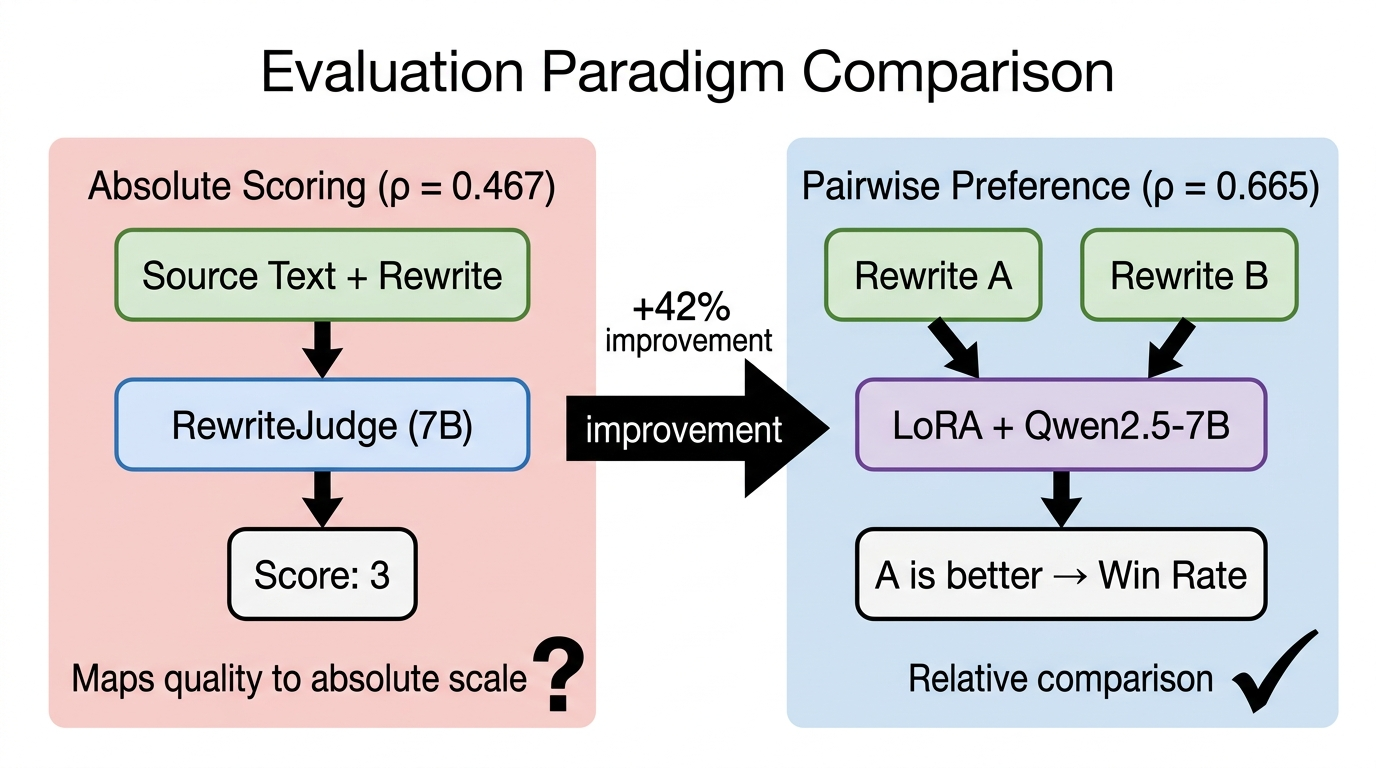
\includegraphics[width=0.9\columnwidth]{figures/ai_generated/pairwise_vs_absolute_v1.png}
\caption{Pairwise preference learning boosts correlation 6.7\% over absolute scoring ($\rho$=0.688 vs.\ 0.645) by predicting relative quality.}
\label{fig:paradigm_comparison}
\end{figure}

\subsection{Method}

We create pairwise training data from 600 samples by pairing rewrites with score differences $\geq 0.67$:
\begin{equation}
    \mathcal{P} = \{(r_i, r_j) \mid |q_i - q_j| \geq 0.67\}
    \label{eq:pairs}
\end{equation}0Pr(=
yielding 2,652 balanced comparisons (1,326 per class). Each example asks the model to identify the higher-quality rewrite. 

At inference, all $\binom{129}{2}=8{,}256$ evaluation pairs are scored; each rewrite's \emph{win rate} is:
\begin{equation}
\small
    \text{WinRate}(r_i) = \frac{1}{N-1} \sum_{j \neq i} \mathbf{1}[\text{Pref}(r_i, r_j) = 1]
    \label{eq:winrate}
\end{equation}
and Spearman correlation is computed between win rates and human average scores.

\subsection{Results}

Table~\ref{tab:pairwise_results} compares absolute scoring and pairwise preference learning against zero-shot LLM baselines.
The pairwise model achieves $\rho$=0.688, a \textbf{6.7\% improvement} over absolute scoring ($\rho$=0.645) and substantially outperforming all zero-shot baselines.
Among zero-shot models, Qwen2.5-72B ($\rho$=0.406) and DeepSeek-V3 ($\rho$=0.391) show moderate positive correlation, while larger and more recent models perform surprisingly poorly: Qwen3-235B ($\rho$=0.132), DeepSeek-V3.1 ($\rho$=$-$0.049), DeepSeek-V3.2 ($\rho$=$-$0.274), GPT-4.1 ($\rho$=$-$0.145) and Kimi-K2 ($\rho$=$-$0.472).
Notably, our 8B fine-tuned model outperforms all zero-shot baselines including models up to 1TB parameters, demonstrating that task-specific fine-tuning with pairwise preference learning is far more effective than scaling model size.

\begin{table}[h]
\centering
\caption{Comparison of evaluation paradigms. Pairwise preference learning substantially outperforms absolute scoring and zero-shot baselines, even against massive frontier models.}
\label{tab:pairwise_results}
\resizebox{0.85\columnwidth}{!}{%
\begin{tabular}{lcc}
\toprule
Method & Params & Spearman $\rho$ \\
\midrule
\textbf{Pairwise (cross-source, ours)} & \textbf{8B} & \textbf{+0.688} \\
Pairwise (cross-source, ours) & 7B & +0.665 \\
Absolute scoring (balanced, ours) & 7B & +0.607 \\
\midrule
Qwen2.5-72B-Instruct (zero-shot) & 72B & +0.406 \\
DeepSeek-V3 (zero-shot) & 685B & +0.391 \\
Qwen3-235B-A22B (zero-shot) & 235B & +0.132 \\
DeepSeek-V3.1-Terminus (zero-shot) & 685B & $-$0.049 \\
GPT-4.1 (zero-shot) & 1.8T & $-$0.145 \\
DeepSeek-V3.2 (zero-shot) & 685B & $-$0.274 \\
Kimi-K2 (zero-shot) & 1T & $-$0.472 \\
\bottomrule
\end{tabular}
}
\end{table}

\subsection{Scaling and Generational Analysis}
\label{sec:scaling}

Figure~\ref{fig:scaling} plots parameter count against Spearman $\rho$ for all pairwise zero-shot baselines. The relationship between scale and evaluation quality is \emph{negative}: larger models do not systematically improve rewriting assessment, with our fine-tuned 7B model being the sole outlier far above the downward trend. 

\begin{figure}[h]
\centering

\includegraphics[width=0.9\columnwidth]{figures/qwen3-8b_and_qwen2.5-7b/scaling_analysis.pdf}
\caption{Model scale vs.\ evaluation quality on RewritingBench. Scaling up zero-shot models does not improve rewriting evaluation; our 8B LoRA model outperforms all zero-shot baselines.}
\label{fig:scaling}
\end{figure}

Within model families (Figure~\ref{fig:generational}), performance often collapses as scale increases: Qwen3-235B ($\rho$=0.132) drops significantly from Qwen2.5-72B ($\rho$=0.406), while DeepSeek's correlation turns negative in later versions (V3.1/V3.2). This regression extends to frontier models like GPT-4.1 ($\rho$=$-0.145$) and Kimi-K2 ($\rho$=$-0.472$), which show the worst alignment despite their size. We hypothesize this reflects a training misalignment: optimization for helpfulness may conflict with the critical judgment needed to distinguish genuine improvements from superficially fluent rewrites.

\begin{figure}[h]
\centering

\includegraphics[width=0.8\columnwidth]{figures/qwen3-8b_and_qwen2.5-7b/generational_regression.pdf}
\caption{Generational regression in zero-shot rewriting evaluation, where Qwen3 drops 67\% relative to Qwen2.5, and the DeepSeek family (V3.1, V3.2) collapses into negative correlation.}
\label{fig:generational}
\end{figure}

\textbf{Cross-source training is essential.}
The pairwise model trained on cross-source pairs ($\rho$=0.665) substantially outperforms the model trained on generated pairs ($\rho$=0.421).
Cross-source pairs, constructed by pairing rewrites from different source texts with different human scores, provide broader quality coverage than generated pairs, which are derived from the same source texts with different generation prompts.

\textbf{Why does pairwise outperform absolute?}
We attribute this to two factors:
(1) pairwise comparison is an inherently easier learning signal than mapping quality to an absolute scale, as the model only needs to detect relative differences rather than learn the full score distribution;
(2) the win-rate aggregation mechanism provides a more robust quality estimate than any single absolute prediction, as each rewrite's score is informed by multiple comparisons.

\subsection{Ablation Studies}
\label{sec:pairwise_ablation}

\subsubsection{LoRA Rank Ablation}

% \begin{table}[t]
% \centering
% \caption{LoRA rank ablation for pairwise preference evaluation. All models trained with cross-source pairs (2,652), 3 epochs, on a single 3090 GPU.}
% \label{tab:lora_rank_ablation}
% \begin{tabular}{cccc}
% \toprule
% Rank $r$ & $\alpha$ & Params & Spearman $\rho$ \\
% \midrule
% 8  & 16 & $\sim$0.1\% & +0.685 \\
% 16  & 32 & $\sim$0.2\% & +0.665 \\
% \textbf{32} & \textbf{64} & $\sim$0.4\% & \textbf{+0.705} \\
% \bottomrule
% \end{tabular}
% \end{table}



Table~\ref{tab:lora_rank_ablation} investigates the sensitivity of pairwise evaluation quality to LoRA rank ($r$). We observe that performance generally scales with rank, with $r=32$ achieving the peak Spearman $\rho$ of 0.705 for Qwen2.5-7B and 0.713 for Qwen3-8B. The narrow performance range across ranks (maximal $\Delta\rho \approx 0.03$) indicates pairwise preference learning is remarkably robust to adapter capacity. Even at the lowest configuration ($r=8$), both models achieve over $\rho=0.67$, outperforming most baselines. For resource-constrained scenarios, $r=8$ offers an optimal trade-off, requiring only $\sim$0.1\% additional parameters (80MB adapter) and significantly reduced training time.

\begin{table}[h]
\centering
\caption{LoRA rank ablation: effect on trainable parameters and Spearman correlation.}
\label{tab:lora_rank_ablation}
\resizebox{0.8\columnwidth}{!}{%
\begin{tabular}{lcccc} % 变成 5 列
\toprule
Model & Rank $r$ & $\alpha$ & Params & Spearman $\rho$ \\
\midrule
\multirow{3}{*}{Qwen2.5-7B} & 8  & 16 & $\sim$0.1\% & +0.685 \\
           & 16 & 32 & $\sim$0.2\% & +0.665 \\
           & \textbf{32} & \textbf{64} & $\sim$0.4\% & \textbf{+0.705} \\
\midrule
\multirow{3}{*}{Qwen3-8B}  & 8  & 16 & $\sim$0.1\% & +0.679 \\
           & 16 & 32 & $\sim$0.2\% & +0.688 \\
           & \textbf{32} & \textbf{64} & $\sim$0.4\% & \textbf{+0.713} \\
\bottomrule
\end{tabular}
}
\end{table}

\subsubsection{Data Efficiency}

% \begin{table}[t]
% \centering
% \caption{Pairwise data efficiency: performance at different fractions of training data (LoRA $r$=16, 3 epochs).}
% \label{tab:pairwise_data_efficiency}
% \begin{tabular}{lcc}
% \toprule
% Training Data & Pairs & Spearman $\rho$ \\
% \midrule
% 25\% & 663  & +0.434 \\
% 50\% & 1,326 & +0.140 \\
% \textbf{100\%} & \textbf{2,652} & \textbf{+0.665} \\
% \bottomrule
% \end{tabular}
% \end{table}


Table~\ref{tab:pairwise_data_efficiency} investigates the scaling behavior of pairwise evaluation quality. We observe a sharp contrast between model families: Qwen3-8B exhibits robust, monotonic scaling, reaching $\rho=0.611$ with only 25\% of the data. In contrast, Qwen2.5-7B shows a non-monotonic anomaly, where performance plummets from $\rho=0.434$ (25\%) to $\rho=0.140$ (50\%) before recovering at 100\% data. We found the root cause: the 50\% model developed a strong \emph{position bias}, consistently predicting that the second presented rewrite is preferred, regardless of content.

\begin{table}[h]
\centering
\small
\caption{Pairwise data efficiency: performance at different fractions of training data (LoRA $r=16$, $3$ epochs) for Qwen3-8B and Qwen2.5-7B.}
\label{tab:pairwise_data_efficiency}
\resizebox{0.8\columnwidth}{!}{%
\begin{tabular}{lccc}
\toprule
Model & Training Data & Pairs & Spearman $\rho$ \\
\midrule
\multirow{3}{*}{Qwen2.5-7B} & 25\% & 663  & +0.434 \\
                            & 50\% & 1,326 & +0.140 \\
                            & \textbf{100\%} & \textbf{2,652} & \textbf{+0.665} \\
\midrule
\multirow{3}{*}{Qwen3-8B}   & 25\% & 663  & +0.611 \\ % 填入你的新数据
                            & 50\% & 1,326 & +0.669 \\
                            & \textbf{100\%} & \textbf{2,652} & \textbf{+0.688} \\
\bottomrule
\end{tabular}
}
\end{table}

Evidence for this bias is captured by two diagnostics. First, the \textbf{accuracy-correlation paradox}: the 50\% model achieves 99.2\% pairwise accuracy yet only $\rho$=0.140, because our accuracy metric counts ties (from position-swap averaging) as correct. The 100\% model achieves 90.0\% accuracy and $\rho$=0.665, where accuracy reflects genuine quality discrimination. Second, \textbf{position-swap averaging}: presenting each pair in both orderings (A,B) and (B,A) and averaging preferences mitigates position bias. A biased model that always predicts ``second rewrite wins'' produces average preference $\approx 0.5$ per pair, collapsing the win-rate distribution and yielding near-zero Spearman correlation. This finding highlights a risk and mitigation: pairwise models can exploit spurious correlations in subsets, but position-swap averaging provides a built-in diagnostic. For practical deployment, we recommend using accuracy-correlation consistency as a validation signal and ensuring sufficient data diversity to prevent shortcut learning.


% ============================================================
\section{Discussion}
\label{sec:discussion}
% ============================================================

\textbf{Why do traditional metrics fail for rewriting?}
Our error analysis (Section~\ref{sec:error_analysis}) traces the universal negative correlation to a fundamental misalignment: overlap-based metrics measure surface similarity to the source, while human judgment evaluates rewrite quality.
For rewriting, where the goal is transformation rather than reproduction, these objectives are inversely correlated.
This finding generalizes beyond Chinese: any evaluation scenario where good outputs should differ from inputs will face the same challenge.

\textbf{Simple output format beats reasoning.}
The surprising superiority of direct scoring ($\rho$=0.645) over chain-of-thought reasoning ($\rho$=0.360) suggests that, at the 8B scale, evaluation capability is better expressed through direct prediction. This aligns with findings that smaller models may lack the capacity for reliable multi-step reasoning~\citep{wang2024vlm}, where forcing explicit reasoning steps introduces performance-degrading noise.

\textbf{Pairwise preference learning is superior for rewriting evaluation.}
The 6.7\% improvement from absolute scoring ($\rho = 0.645$) to pairwise preference learning ($\rho = 0.688$) demonstrates that rewriting quality judgment is inherently relative. This is consistent with recent findings in general NLP evaluation \citep{kim2024prometheus2, lee2025reliable}, where pairwise comparisons have been shown to provide more robust and human-aligned evaluations. 

Our contribution is demonstrating this effect specifically for Chinese text rewriting, where the gap between pairwise and absolute is particularly large due to the difficulty of the absolute scoring task. Notably, accuracy alone is a misleading proxy: as shown in Figure~\ref{fig:acc_vs_rho}, Qwen3-235B achieves 72.0\% pairwise accuracy yet only $\rho = 0.132$, while our fine-tuned 8B model achieves $\rho = 0.688$ with consistent accuracy--correlation alignment (see Appendix~\ref{sec:appendix_acc_rho} for full analysis).

\begin{figure}[h]
\centering

\includegraphics[width=0.95\columnwidth]{figures/qwen3-8b_and_qwen2.5-7b/accuracy_vs_rho.pdf}
\caption{Pairwise accuracy vs.\ Spearman $\rho$: high accuracy but low $\rho$ shows accuracy can mislead for zero-shot evaluators}
\label{fig:acc_vs_rho}
\end{figure}

\textbf{Class balancing is essential for score prediction.}
The dramatic difference between balanced ($\rho$=0.645) and unbalanced ($\rho$=0.337) training underscores the importance of class balance in ordinal prediction tasks.
Without balancing, the model learns to predict the majority class (Score~1), achieving 82\% mode collapse.
This is a common challenge in ordinal regression~\citep{fernandez2018learning}, and our oversampling strategy provides an effective solution.

\textbf{Ranking vs.\ calibration.}
Our evaluation focuses on ranking correlation (Spearman $\rho$), which measures whether the evaluator correctly orders rewrites by quality.
We note that ranking agreement does not guarantee calibration: the evaluator may systematically over- or under-predict scores while maintaining correct relative ordering.
For benchmark purposes, ranking correlation is the primary concern, as it determines whether the evaluator can reliably distinguish high-quality from low-quality rewrites.
Calibration improvements (e.g., through temperature tuning or score normalization) are orthogonal to our contribution and can be applied on top of our approach.

\textbf{Correlation vs.\ absolute error.}
RewriteJudge achieves Spearman $\rho$=0.645 with MAE=0.91 on a 0--5 scale.
While the MAE may appear moderate, it reflects a known property of rank-correlation metrics: Spearman $\rho$ measures the \emph{ordinal agreement} between predicted and true rankings, which can be high even when absolute predictions are noisy.
Specifically, an evaluator that consistently overestimates scores by 1 point would have MAE$\approx$1.0 but perfect Spearman correlation ($\rho$=1.0).
In our setting, the moderate MAE (0.91) combined with positive Spearman (0.645) indicates that RewriteJudge captures the correct relative ordering while exhibiting some calibration drift, a common phenomenon in fine-tuned evaluators~\citep{lee2025reliable}.
For practical applications such as data filtering (Section~\ref{sec:downstream_results}), ranking accuracy is more important than absolute score precision, as the goal is to select the best rewrites rather than predict their exact quality scores.

\textbf{Limitations.}
Our work has several limitations. First, the training set of 730 pairs (1,008 after balancing) is small and only covers Chinese, so performance and cross-lingual generalization may improve with more data. Second, we use LoRA for efficiency (16 min on a single H20 GPU); full-parameter fine-tuning could yield higher performance but needs more resources. Finally, our scope is limited to general-purpose improvement; future work should cover specialized tasks like style transfer or simplification.

% ============================================================
\section{Conclusion}
\label{sec:conclusion}
% ============================================================

We present RewritingBench, the first human-annotated benchmark for Chinese text rewriting, featuring 730 annotated pairs. Our analysis reveals that traditional metrics correlate negatively with human judgment due to a fundamental misalignment between overlap and quality. To address this, we demonstrate that pairwise preference learning provides a superior framework: a fine-tuned 8B model achieves $\rho=0.688$, significantly outperforming absolute scoring ($\rho=0.645$), zero-shot models up to 235B parameters ($\rho \leq 0.406$), and specialized evaluators(Prometheus~2: $\rho$=0.124). Downstream validation confirms that our evaluator-guided filtering improves data quality by 47\% over random selection. Our benchmark and findings provide a foundation for Chinese rewriting evaluation. We release our data, code, and fine-tuned models to support future research.

\textbf{Future work.}
We plan to expand RewritingBench to include diverse tasks (e.g., style transfer, simplification), additional languages, and sophisticated aggregation methods like Bradley-Terry models. We also aim to investigate if the negative correlation between overlap and quality persists across other languages and domains.

% ============================================================
% REFERENCES
% ============================================================

\bibliography{refs}

% ============================================================
% APPENDIX
% ============================================================
\appendix

\section{Training Configuration Details}
\label{sec:appendix_training}

Table~\ref{tab:training_config} summarizes the training configuration for \textsc{RewriteJudge}. We employ Low-Rank Adaptation (LoRA) to fine-tune the model, injecting trainable matrices into seven target modules: query, key, value, output projection, and the three MLP layers (gate, up, and down projections). This configuration results in trainable parameters totaling approximately 0.2\% of the full model.

\subsection{Hyperparameters}
The LoRA adapters are configured with rank $r=16$, scaling factor $\alpha=32$, and a dropout rate of 0.05. We fine-tune the model for 3 epochs using a learning rate of $2 \times 10^{-4}$ with a cosine decay schedule (3\% warmup). The training utilizes 4-bit NF4 quantization and bf16 mixed precision to optimize memory efficiency. With a batch size of 4 and 4 gradient accumulation steps (effective batch size 16), the total training time is approximately 16 minutes on a single NVIDIA H20 GPU.

\begin{table}[h]
\centering
\caption{Complete training configuration for RewriteJudge.}
\label{tab:training_config}
\resizebox{\columnwidth}{!}{%
\begin{tabular}{ll}
\toprule
Hyperparameter & Value \\
\midrule
Base model & Qwen3-8B, Qwen2.5-7B-Instruct \\
Quantization & 4-bit NF4 (double quantization) \\
LoRA rank ($r$) & 16 \\
LoRA scaling ($\alpha$) & 32 \\
LoRA dropout & 0.05 \\
Target modules & q\_proj, k\_proj, v\_proj, o\_proj, \\
 & gate\_proj, up\_proj, down\_proj \\
Learning rate & $2 \times 10^{-4}$ \\
LR scheduler & Cosine (warmup 3\%) \\
Epochs & 3 \\
Batch size & 4 (gradient accumulation: 4) \\
Effective batch size & 16 \\
Precision & bf16 \\
Gradient checkpointing & Enabled \\
Training samples & 1,008 (168 per class) \\
GPU & 1$\times$ NVIDIA H20 GPU (96GB) \\
Training time & $\sim$16 minutes \\
\bottomrule
\end{tabular}
}
\end{table}


\section{Extended Results}
\label{sec:appendix_results}

\subsection{Learning Curve with All Methods}
\label{sec:appendix_full_learning}

% \begin{table}[t]
% \centering
% \caption{Learning curve: Spearman $\rho$ at different training data sizes (class-balanced oversampling).}
% \label{tab:learning_curve}
% \begin{tabular}{lc}
% \toprule
% Samples & $\rho$ \\
% \midrule
% 50 & $-$0.021 \\
% 100 & +0.058 \\
% 200 & +0.189 \\
% 400 & +0.211 \\
% \textbf{1,008} & \textbf{+0.467} \\
% \bottomrule
% \end{table}

Table~\ref{tab:learning_curve} and Figure~\ref{fig:learning_curve_full} illustrate the scaling behavior of evaluation quality relative to training data size. Performance improves monotonically from 50 to 1,008 samples, with a notable inflection point appearing beyond 400 samples. Notably, with as few as 100 balanced samples, RewriteJudge achieves $\rho=0.117$, already outperforming all zero-shot baselines and general-purpose evaluators.
The sustained upward trajectory at the full dataset size suggests that reaching a critical mass of examples per score class (approximately 168 samples) is essential for the model to internalize the subtle semantic distinctions required for high-quality rewriting evaluation.


\begin{table}[h]
\centering
\caption{Learning curve comparison between Qwen2.5-7B and Qwen3-8B evaluators.}
\label{tab:learning_curve}
\resizebox{0.9\columnwidth}{!}{%
\begin{tabular}{lcc}
\toprule
Samples &  $\rho$ (Qwen2.5-7B) &  $\rho$ (Qwen3-8B) \\
\midrule
50 & $-$0.026 & $+$0.058 \\
100 & $+$0.094 & $+$0.117 \\
200 & $+$0.259 & $+$0.136 \\
400 & $+$0.235 & $+$0.247 \\
1008 (full) & $+$0.580 & $+$0.645 \\
\bottomrule
\end{tabular}
}
\end{table}
% \begin{figure}[t]
% \centering
% 
\includegraphics[width=\columnwidth]{figures/qwen3-8b_and_qwen2.5-7b/learning_curve_lora_only.pdf}
% \caption{Learning curve for RewriteJudge. Performance scales monotonically with training data size, with a sharp improvement at 1,008 balanced samples.}
% \label{fig:learning_curve}
% \end{figure}

\begin{figure}[h]
\centering

\includegraphics[width=\columnwidth]{figures/qwen3-8b_and_qwen2.5-7b/learning_curve.pdf}
\caption{Full learning curve including both LoRA variants and baseline methods (dashed lines). All baselines show flat or negative correlation regardless of data size.}
\label{fig:learning_curve_full}
\end{figure}


\subsection{Score Distribution Analysis}

Figure~\ref{fig:score_distribution} illustrates the score frequency across different evaluators. We observe that Zero-shot 7B exhibits an extreme ceiling effect, with over 80\% of its predictions concentrated at Score~4, failing to distinguish between quality levels. Prometheus~2 shows a sharp peak at Score~3, largely ignoring both the lower and upper ends of the spectrum. In contrast, \textsc{RewriteJudge} (both Qwen3-8B and Qwen2.5-7B variants) produces a distribution that closely mirrors the human ground truth across all six score levels, validating the effectiveness of our class-balanced fine-tuning in regularizing the evaluator's output range.

\begin{figure}[h]
\centering

\includegraphics[width=\columnwidth]{figures/qwen3-8b_and_qwen2.5-7b/score_distribution.pdf}
\caption{Distribution of human annotations and RewriteJudge predictions. The balanced training successfully aligns the predicted distribution with human scores.}
\label{fig:score_distribution}
\end{figure}


\subsection{Confusion Matrix Analysis}

Figures~\ref{fig:confusion_lora_qwen3-8b}, \ref{fig:confusion_lora_qwen2.5-7b}, and \ref{fig:confusion_prometheus} provide a granular view of evaluator errors.
Both \textsc{RewriteJudge} variants exhibit a strong diagonal trend consistent with human judgment.
The Qwen3-8B variant correctly identifies 60\% of Score~0 samples and 66.7\% of Score~5 samples, and shows a clear upper-left-to-lower-right diagonal structure with very few extreme misclassifications (e.g., predicting Score~5 for a human Score~0).
The Qwen2.5-7B variant similarly concentrates predictions along the diagonal: 50\% accuracy for Score~0, 58.3\% for Score~4, with the model showing particular strength in the mid-to-high range.
Both variants rarely commit "extreme" errors, confirming that class-balanced fine-tuning preserves ordinal structure.

In stark contrast, Prometheus~2 exhibits a near-total collapse in discriminative power: it predicts Score~3 for 63.6\%--73.9\% of all samples across every human score category, regardless of true quality. This severe mode collapse explains its low Spearman correlation ($\rho$=0.124), as it effectively acts as a constant-score predictor that fails entirely to capture ordinal variance in human judgments.

\begin{figure}[h]
\centering

\includegraphics[width=\columnwidth]{figures/qwen3-8b_and_qwen2.5-7b/confusion_matrix_lora_balanced_simple.pdf}
\caption{Confusion matrix for RewriteJudge(Qwen3-8B) predictions vs.\ human average scores (rounded). The model shows strongest agreement for extreme scores (0 and 4--5).}
\label{fig:confusion_lora_qwen3-8b}
\end{figure}

\begin{figure}[h]
\centering

\includegraphics[width=\columnwidth]{figures/qwen3-8b_and_qwen2.5-7b/confusion_matrix_lora_balanced_simple_qwen2_5_7b_instruct_20260511_200253}
\caption{Confusion matrix for RewriteJudged(Qwen2.5-7B) predictions vs.\ human average scores (rounded). The model shows strongest agreement for extreme scores (0 and 4--5).}
\label{fig:confusion_lora_qwen2.5-7b}
\end{figure}

\begin{figure}[h]
\centering

\includegraphics[width=\columnwidth]{figures/qwen3-8b_and_qwen2.5-7b/confusion_matrix_prometheus2.pdf}
\caption{Confusion matrix for Prometheus~2. The model shows a strong tendency to predict low scores, with most predictions concentrated around Score~1--2.}
\label{fig:confusion_prometheus}
\end{figure}


% \subsection{Inter-Evaluator Agreement}
% \label{sec:appendix_agreement}

% \begin{figure}[t]
% \centering
% 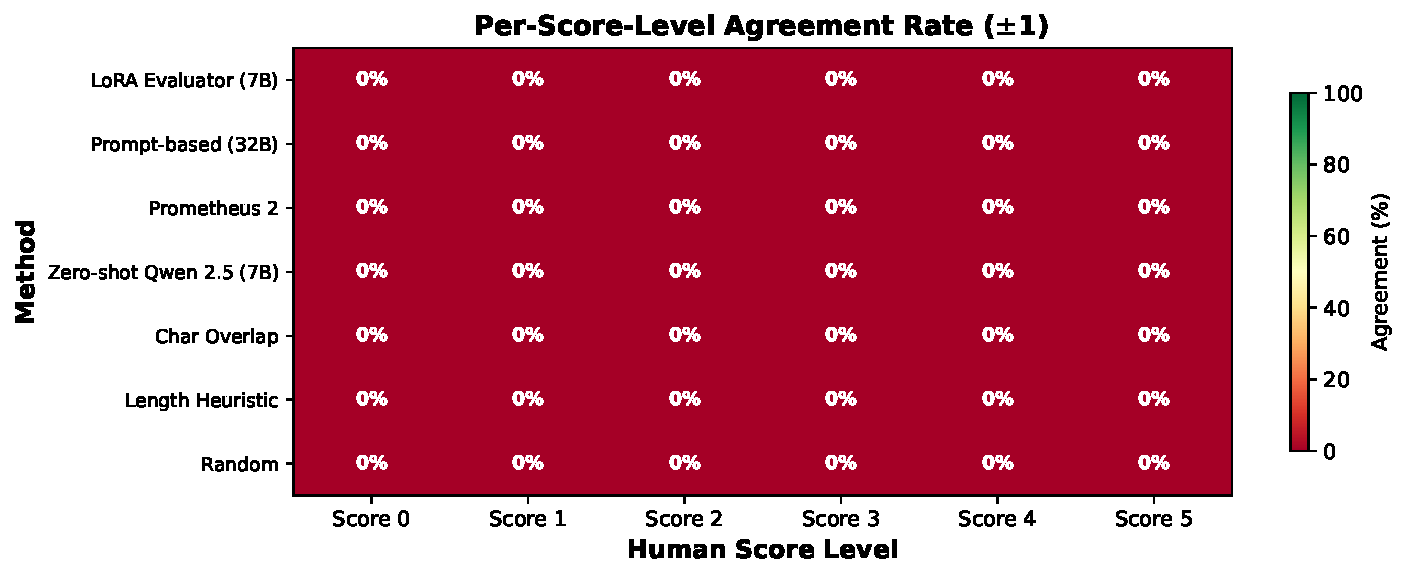
\includegraphics[width=0.9\columnwidth]{figures/agreement_heatmap.pdf}
% \caption{Pairwise Spearman correlation between human annotators and evaluator methods. Human--human agreement ($\sim$0.86) provides an approximate upper bound for evaluator performance.}
% \label{fig:agreement_heatmap}
% \end{figure}

% Figure~\ref{fig:agreement_heatmap} shows the pairwise agreement between all evaluation methods.
% The inter-annotator Spearman correlation of approximately 0.86 provides a practical upper bound for evaluator performance, as individual annotator disagreements set a ceiling on achievable correlation with the average score.

% \begin{figure}[t]
% \centering
% 
\includegraphics[width=\columnwidth]{figures/length_bias_scatter.pdf}
% \caption{Scatter plot of evaluator score vs.\ output text length. RewriteJudge shows no systematic length--score relationship, while traditional metrics show strong positive bias.}
% \label{fig:length_scatter}
% \end{figure}


% \subsection{Delta Improvement Analysis}

% \begin{figure}[t]
% \centering
% 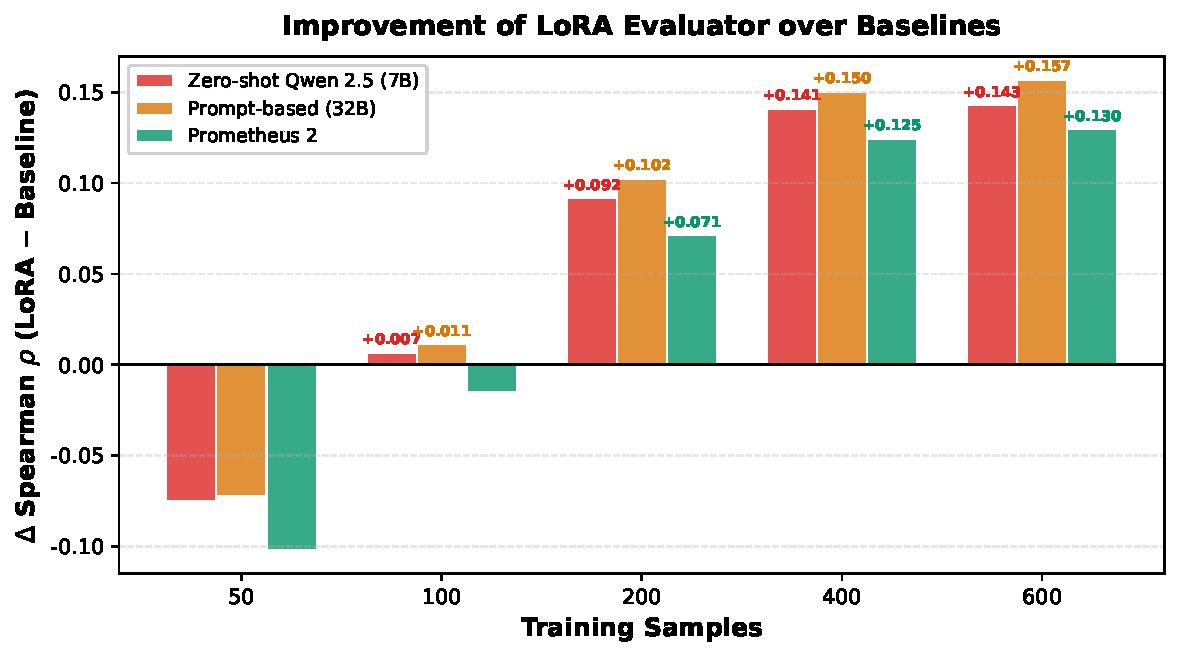
\includegraphics[width=\columnwidth]{figures/delta_improvement.pdf}
% \caption{Per-method improvement analysis showing the delta between method performance and a random baseline across different score ranges.}
% \label{fig:delta_improvement}
% \end{figure}

\section{Extended Bias Analysis}
\label{sec:bias}

% \begin{table}[t]
% \centering
% \caption{Bias analysis across evaluator methods. Lower absolute values indicate less bias. \textbf{LoRA} = RewriteJudge.}
% \label{tab:bias_analysis}
% \resizebox{\columnwidth}{!}{%
% \begin{tabular}{lccccc}
% \toprule
% Method & Output Len.\,$r$ & Input Len.\,$r$ & Verbosity $\rho$ & Pos.\,Bias $r$ & Avg \\
% \midrule
% \textbf{RewriteJudge} & $\mathbf{-0.05}$ & $\mathbf{-0.07}$ & $\mathbf{-0.09}$ & $\mathbf{-0.07}$ & $\mathbf{0.07}$ \\
% Prometheus~2 & $-$0.06 & $-$0.07 & $-$0.06 & +0.04 & 0.06 \\
% Char Overlap & +0.27 & +0.19 & +0.21 & +0.20 & 0.22 \\
% Length Heuristic & +0.23 & $-$0.04 & +0.86 & +0.79 & 0.48 \\
% \bottomrule
% \end{tabular}
% }
% \end{table}


A reliable evaluator should judge quality based on content, not spurious features such as text length or verbosity.
Table~\ref{tab:bias_analysis} compares bias across six methods along four dimensions: output length bias, input length bias, verbosity bias, and position bias.
We include two additional reference methods: (1) \textbf{character overlap} (JACCARD-CHAR), representing traditional overlap-based metrics; and (2) a \textbf{length heuristic} that assigns quality scores based solely on the ratio of rewrite length to source length, a naive but surprisingly common proxy used in practice.


\begin{table}[h]
\centering
\small
\footnotesize % 1. 调整字号
\setlength{\tabcolsep}{3pt} % 2. 压缩列间距
\caption{Bias analysis for different evaluator methods. Lower absolute correlation values indicate less bias.}
\label{tab:bias_analysis}
\resizebox{\columnwidth}{!}{%
\begin{tabular}{lccccc}
\toprule
Method & Output Len. $r$ & Input Len. $r$ & Verbosity $\rho$ & Pos. Bias $r$ & Bias Score \\
\midrule
RewriteJudge (Ours, Qwen3-8B) & -0.033 & -0.070 & 0.006 & 0.120 & 0.057 \\
RewriteJudge (Ours, Qwen2.5-7B) & -0.058 & -0.115 & 0.106 & 0.187 & 0.116 \\
Prometheus 2 & 0.010 & -0.071 & 0.098 & 0.223 & 0.100 \\
Zero-shot Qwen3-8B & 0.325 & 0.167 & 0.382 & 0.437 & 0.328 \\
Char Overlap & 0.306 & 0.044 & 0.760 & 0.762 & 0.468 \\
Length Heuristic & 0.287 & 0.052 & 0.741 & 0.681 & 0.441 \\
\bottomrule
\end{tabular}
}
\end{table}



\textbf{Length bias}
Both RewriteJudge variants show minimal output length bias (Qwen3-8B: $r=-0.033$; Qwen2.5-7B: $r=-0.058$), well below Zero-shot Qwen3-8B ($r=0.325$), character overlap ($r=0.306$), and the length heuristic ($r=0.287$). Prometheus~2 shows near-zero output length bias ($r=0.010$) but moderate input length bias ($r=-0.071$). Figure~\ref{fig:length_quartile} visualizes this across output length quartiles: both RewriteJudge variants maintain a near-flat or slightly non-monotonic trajectory (peaking at Q2--Q3 and declining at Q4), while Zero-shot Qwen3-8B, Prometheus~2, character overlap, and the length heuristic all exhibit clear monotonic upward trends, systematically rewarding longer outputs regardless of quality. The length heuristic, in particular, exhibits extreme verbosity bias ($\rho=0.741$), confirming a known failure mode where naive metrics struggle to distinguish between informative expansion and redundant verbosity~\citep{kuang2024evaluating}.

\begin{figure}[h]
\centering

\includegraphics[width=\columnwidth]{figures/qwen3-8b_and_qwen2.5-7b/length_quartile_trend.pdf}
\caption{Mean evaluator score by output length quartile. RewriteJudge maintains consistent scores across quartiles, while traditional metrics show increasing scores for longer outputs.}
\label{fig:length_quartile}
\end{figure}

\textbf{Position bias}
RewriteJudge maintains low position bias across both variants (Qwen3-8B: $r=0.120$; Qwen2.5-7B: $r=0.187$), while Zero-shot Qwen3-8B shows substantially higher position bias ($r=0.437$).
The length heuristic ($r=0.681$) and character overlap ($r=0.762$) show the most extreme position bias, suggesting their scores are heavily influenced by input-output length differences rather than rewrite quality.
Figure~\ref{fig:bias_radar} summarizes all four bias dimensions in a radar chart: both RewriteJudge variants cluster near the center (Bias Score: 0.057 and 0.116), while Zero-shot Qwen3-8B (0.328), character overlap (0.468), and the length heuristic (0.441) occupy substantially larger areas, reflecting high bias across multiple dimensions.

\begin{figure}[h]
\centering

\includegraphics[width=\columnwidth]{figures/qwen3-8b_and_qwen2.5-7b/bias_radar.pdf}
\caption{Radar chart comparing bias dimensions across evaluators. RewriteJudge shows consistently low bias across all measured dimensions.}
\label{fig:bias_radar}
\end{figure}

% Figure~\ref{fig:bias_radar} visualizes the bias profile across dimensions, confirming that RewriteJudge maintains low bias comparable to Prometheus~2 while substantially outperforming it in correlation with human judgments.

\begin{figure}[h]
\centering

\includegraphics[width=\columnwidth]{figures/qwen3-8b_and_qwen2.5-7b/verbosity_bias_bars.pdf}
\caption{Verbosity bias comparison. RewriteJudge shows near-zero verbosity bias, while the length heuristic exhibits extreme preference for verbose outputs ($\rho$=0.741).}
\label{fig:verbosity_bias}
\end{figure}

\textbf{Verbosity bias.}
Figure~\ref{fig:verbosity_bias} breaks down verbosity bias by output-to-input length ratio across two categories present in our evaluation set: Concise (ratio $<$0.8) and Similar (0.8--1.2).
RewriteJudge variants assign consistently low scores in both categories (Qwen3-8B: Concise 1.7, Similar 1.9, $\Delta$=0.2; Qwen2.5-7B: Concise 1.4, Similar 2.0, $\Delta$=0.6), remaining well below all other methods in absolute score level.
In contrast, other methods show substantially larger Concise-to-Similar gaps: length heuristic (1.7 $\rightarrow$ 2.4, $\Delta$=0.7), and character overlap shows the largest jump (3.4 $\rightarrow$ 4.6, $\Delta$=1.2), reflecting strong systematic preference for longer outputs.
The verbosity bias scores in Table~\ref{tab:bias_analysis} confirm this: RewriteJudge Qwen3-8B achieves near-zero verbosity bias ($\rho=0.006$), far below Zero-shot Qwen3-8B ($\rho=0.382$), character overlap ($\rho=0.760$), and the length heuristic ($\rho=0.741$).
\section{Extended Zero-Shot Baseline Analysis}
\label{sec:appendix_zero_shot}

\subsection{Accuracy vs.\ Ranking Correlation}
\label{sec:appendix_acc_rho}

A natural expectation is that higher pairwise accuracy should correspond to higher Spearman $\rho$.
Our results contradict this: Table~\ref{tab:acc_rho_paradox} shows that pairwise accuracy and ranking correlation are poorly aligned for zero-shot models.

\begin{table}[h]
\centering
\caption{Accuracy--correlation paradox in zero-shot pairwise evaluation. Qwen3-235B achieves the highest accuracy (72.0\%) but near-zero $\rho$=0.132.}
\label{tab:acc_rho_paradox}
\resizebox{\columnwidth}{!}{%
\begin{tabular}{lccc}
\toprule
Model & Accuracy (\%) & Spearman $\rho$ & Paradox? \\
\midrule
Ours (8B LoRA) & 69.5 & +0.688 & No \\
Ours (7B LoRA) & 90.0 & +0.665 & No \\
Qwen3-235B & 72.0 & +0.132 & Yes \\
Qwen2.5-72B & 69.3 & +0.406 & Mild \\
DeepSeek-V3 & 67.7 & +0.391 & No \\
DeepSeek-V3.1 & 49.9 & $-$0.049 & Yes \\
Kimi-K2 & 31.6 & $-$0.472 & No \\
\bottomrule
\end{tabular}
}
\end{table}

As visualized in Figure~\ref{fig:acc_vs_rho}, Qwen3-235B achieves high zero-shot accuracy (72.0\%) yet fails to provide a meaningful ranking ($\rho=0.132$). This paradox suggests that zero-shot models may correctly identify "easy" pairs with large quality gaps but fail to maintain consistent logic across the full spectrum. Our fine-tuned model variants effectively resolve this, as seen by their positioning in the top-right "High Accuracy, High $\rho$" quadrant.



\subsection{Format Compliance vs.\ Evaluation Quality}
\label{sec:appendix_parse}

We examine whether format compliance (the ability to follow the pairwise comparison output format) correlates with evaluation quality.
Table~\ref{tab:parse_analysis} shows the parse failure rate for each zero-shot baseline.

\begin{table}[h]
\centering
\caption{Format compliance vs.\ evaluation quality. Models with zero parse failures include both the best and worst performers, indicating format compliance is independent of evaluation capability.}
\label{tab:parse_analysis}
\resizebox{\columnwidth}{!}{%
\begin{tabular}{lccc}
\toprule
Model & Parse Fail (\%) & Spearman $\rho$ & Quality \\
\midrule
DeepSeek-V3 & 0.0 & +0.391 & Best zero-shot \\
Kimi-K2 & 0.0 & $-$0.472 & Worst zero-shot \\
DeepSeek-V3.1 & 0.0 & $-$0.049 & Poor \\
DeepSeek-v3.2 & 0.0 & -0.274 & Poor  \\
GPT-4.1 & 0.0 & -0.145 &  Poor  \\
Qwen2.5-72B & 8.8 & +0.406 & Good \\
Qwen3-235B & 9.0 & +0.132 & Poor \\
\bottomrule
\end{tabular}
}
\end{table}

The results in Figure~\ref{fig:parse_vs_rho} confirm that format compliance and evaluation quality are \textbf{orthogonal}. Models with 100\% compliance (0\% failure) span the entire performance spectrum, from the best zero-shot baseline (DeepSeek-V3) to the worst (Kimi-K2). This indicates that the mechanical ability to follow instructions is independent of the critical capacity to judge text quality.

\begin{figure}[h]
\centering

\includegraphics[width=\columnwidth]{figures/qwen3-8b_and_qwen2.5-7b/parse_failure_vs_rho.pdf}
\caption{Parse failure rate vs.\ Spearman $\rho$. No correlation exists between format compliance and evaluation quality: models with 0\% parse failures span the full quality range.}
\label{fig:parse_vs_rho}
\end{figure}

\section{Chinese Annotation Examples}
\label{sec:appendix_examples}

To provide a qualitative understanding of the benchmark, Table~\ref{tab:examples} presents several representative cases covering various quality levels. These examples illustrate the nuances of Chinese text rewriting, ranging from simple lexical substitutions to sophisticated stylistic enhancements. We observe that \textsc{RewriteJudge} (RJ) predictions align closely with human gold standard scores, successfully capturing subtle improvements in fluency and expressiveness while remaining sensitive to instances where the rewrite fails to provide significant added value.

\begin{table}[h]
\centering
\caption{Representative examples from the evaluation benchmark. \textbf{Source}: original text; \textbf{Rewrite}: model-generated rewrite; \textbf{Human}: average human score; \textbf{RJ}: RewriteJudge prediction.}
\label{tab:examples}
\resizebox{\columnwidth}{!}{%
\begin{tabular}{p{0.25\columnwidth}p{0.4\columnwidth}cc}
\toprule
Source & Rewrite & Human & RJ \\
\midrule
今天天气很好，我们决定去公园散步。 &
阳光明媚，微风轻拂，我们来到公园漫步，享受这惬意的时光。 &
4 & 4 \\
\midrule
这个问题的解决方案需要进一步研究。 &
要解决此事还需深入探究才能找到答案。 &
2 & 2 \\
\midrule
他是一个非常好的学生，学习成绩优异。 &
他学习刻苦努力，是个品学兼优的好学生。 &
3 & 3 \\
\midrule
这家餐厅的菜很好吃。 &
这儿的菜品味道鲜美可口，令人回味无穷。 &
3 & 2 \\
\midrule
会议上讨论了关于环保的问题。 &
大家在会议中就环境保护议题展开了深入探讨。 &
4 & 4 \\
\bottomrule
\end{tabular}
}
\end{table}


% ============================================================
\section{Error Analysis: Why Traditional Metrics Fail}
\label{sec:error_analysis}
% ============================================================

The results so far have demonstrated that pairwise preference learning substantially outperforms both traditional metrics and absolute scoring. In this section, we turn to diagnosing \emph{why traditional metrics fail so dramatically on the rewriting task.}
The universal negative correlation of traditional metrics with human judgment is the most striking finding of our benchmark.
In this section, we provide a detailed diagnosis.

\subsection{Two Error Patterns}

We identify two systematic error patterns that explain the negative correlations:

\textbf{Pattern 1: Surface similarity without quality.}
Rewrites that are near-copies of the source text, changing only a few words while preserving the original structure, receive high overlap-based metric scores but low human ratings.
For example, a rewrite that substitutes ``\textit{加盟}'' with ``\textit{加盟后}'' and ``\textit{场场}'' with ``\textit{几乎每场}'' achieves BLEU=0.55 but receives a human score of only 0.7.
The metric rewards lexical overlap that reflects copying, not genuine quality improvement.

\textbf{Pattern 2: Quality without surface similarity.}
High-quality rewrites that substantially restructure the sentence, using different vocabulary and syntax while preserving meaning, receive near-zero metric scores but high human ratings.
A rewrite that restructures a passage about a press conference into a more concise summary achieves BLEU=0.00 but receives a human score of 4.0.
The metric penalizes the very lexical variation that characterizes successful rewriting.

\subsection{Root Cause: Misaligned Objectives}

These two patterns reveal a fundamental misalignment: overlap-based metrics measure how \emph{similar} a rewrite is to its source, while human judgment evaluates how \emph{good} the rewrite is.
The critical insight is that these are not merely different metrics; they are \emph{inversely correlated} for rewriting.
Pattern~1 shows that high source similarity indicates \emph{insufficient transformation} (the rewrite barely changed anything), while Pattern~2 shows that high source dissimilarity indicates \emph{successful transformation} (the rewrite substantially improved the text).
This inverse relationship explains why the negative correlations are universal and statistically significant rather than reflecting random noise or a specific metric deficiency.
For text rewriting, a task where the goal is to differ from the source while preserving meaning, these two objectives are inversely correlated.
This explains why the strongest negative correlations are observed for character-level metrics (JACCARD-CHAR: $\rho$=$-$0.60), which most directly measure surface overlap, while semantic metrics like SBERT-COSINE ($\rho$=$-$0.28) show somewhat weaker (but still significantly negative) correlations.

\subsection{Implications}

This finding has practical implications: researchers developing or evaluating Chinese rewriting systems cannot rely on any existing automatic metric for quality assessment.
Our RewritingBench and the associated pairwise preference evaluator provide a validated alternative.

\section{Scoring Prompts for LLM and Human Evaluation}
\label{sec:appendix_prompts} 

We investigate how prompt detail affects evaluation quality by comparing three variants: \textbf{Simple} (minimal), \textbf{Standard} (brief criteria), and \textbf{Detailed} (fine-grained rubrics). Notably, the \textbf{Detailed} prompt exactly matches our benchmark's human rubric, grounding the model directly in the human annotation protocol.


\medskip
\noindent\textbf{Simple prompt}
\medskip

\begin{prompttextbox}{Simple prompt}{simple}
\small
请帮我评判输入文本和输出文本重写的质量，并给出最终综合评分（0-5分的整数）。
\end{prompttextbox}

\medskip
\noindent\textbf{Standard prompt}
\medskip

\begin{prompttextbox}{Standard prompt}{standard}
\small
你是一个专业的中文文本改写质量评估专家。请根据以下维度对中文文本改写质量进行评分（0-5分）：

\medskip\textbf{评分维度：}
\begin{itemize}[leftmargin=1.2em,itemsep=0pt,topsep=2pt]
  \item 语义一致性：改写是否保留了原文的核心语义
  \item 句式重构：改写是否进行了句法结构的改变
  \item 词汇变化：改写是否使用了不同的词汇表达
  \item 风格保持：改写是否保持了原文的风格和长度
\end{itemize}

\medskip\textbf{评分标准：}
\begin{itemize}[leftmargin=1.2em,itemsep=0pt,topsep=2pt]
  \item 0分：改写完全失败（严重语义扭曲或毫无改写）
  \item 1分：改写质量很差 
  \item 2分：改写质量较差 
  \item 3分：改写质量一般
  \item 4分：改写质量较好 
  \item 5分：改写质量优秀
\end{itemize}

\medskip
请先简要分析，然后给出最终综合评分（0-5分的整数）。
\end{prompttextbox}

\medskip
\noindent\textbf{Detailed prompt}
\medskip

\begin{prompttextbox}{Detailed prompt --- identical to human annotation rubric}{detailed}
\small
请帮我判断输入文本与输出文本是否满足以下要求：
\begin{itemize}[leftmargin=1.2em,itemsep=2pt,topsep=2pt]
  \item \textbf{要求1.} 在保持原文含义不变的前提下，用原文不同的文字进行表达，不额外新增、删减会严重影响语义的内容。
  \item \textbf{要求2.} 在保证逻辑正确、语序通顺的前提下，变换实体、短语、概念出现的前后顺序、结构关系；顺序变换幅度越小，分数越低。
  \item \textbf{要求3.} 在保证特殊实体、引用、解释、特定语句不变的前提下，使用同义词替换；同义词替换越少，分数越低。
  \item \textbf{要求4.} 保持与原文语言风格一致，字数长度变化合理；语言风格差距越大，分数越低。
  \item \textbf{要求5.} 改写综合评分要非常严格，同时考虑上述4个要求；在保证语义一致（要求1）的前提下，（要求2,3）变化越大越好，字数越接近越好（要求4）；如果存在大量长字段完全复制，则给0分。
\end{itemize}

\medskip
评分准则，每个要求最低0分，满分均为5分，评分要尽可能严格。
\end{prompttextbox}



As shown in Table~\ref{tab:prompt_granularity}, performance improves monotonically with prompt granularity.
The detailed prompt achieves $\rho=0.645$, outperforming the standard prompt by 6.2\% and the simple prompt by 27.2\%.
This suggests that explicitly providing the four evaluation dimensions during fine-tuning helps the model internalize the annotation criteria and better align its predictions with human judgment.
The substantial gap between simple and detailed ($\Delta\rho=0.138$) indicates that the scoring rubric is not merely redundant context, but carries essential information about what constitutes quality in Chinese text rewriting.


\begin{table}[h]
\centering
\caption{Effect of prompt granularity on evaluation quality (Qwen3-8B, balanced training).}
\label{tab:prompt_granularity}
\resizebox{0.75\columnwidth}{!}{%
\begin{tabular}{lc}
\toprule
Prompt Variant & Spearman $\rho$ \\
\midrule
Simple prompt & $+$0.507 \\
Standard prompt & $+$0.607 \\
\textbf{Detailed prompt} & $\mathbf{+0.645}$ \\
\bottomrule
\end{tabular}
}
\end{table}





\end{document}
